
\documentclass{beamer}
\usepackage{media9}
\usepackage{listings}

\mode<presentation> {

%\usetheme{default}
%\usetheme{AnnArbor}
%\usetheme{Antibes}
%\usetheme{Bergen}
%\usetheme{Berkeley}
%\usetheme{Berlin}
%\usetheme{Boadilla}
%\usetheme{CambridgeUS}
%\usetheme{Copenhagen}
%\usetheme{Darmstadt}
%\usetheme{Dresden}
%\usetheme{Frankfurt}
%%\usetheme{Goettingen}
%\usetheme{Hannover}
%\usetheme{Ilmenau}
%\usetheme{JuanLesPins}
%\usetheme{Luebeck}
%\usetheme{Madrid}
%\usetheme{Malmoe}
%\usetheme{Marburg}
%\usetheme{Montpellier}
%\usetheme{PaloAlto}
%\usetheme{Pittsburgh}
\usetheme{Rochester}
%\usetheme{Singapore}
%\usetheme{Szeged}
%\usetheme{Warsaw}


%\usecolortheme{albatross}
%\usecolortheme{beaver}
%\usecolortheme{beetle}
%\usecolortheme{crane}
%\usecolortheme{dolphin}
%\usecolortheme{dove}
%\usecolortheme{fly}
\usecolortheme{lily}
%\usecolortheme{orchid}
%\usecolortheme{rose}
%\usecolortheme{seagull}
%\usecolortheme{seahorse}
%\usecolortheme{whale}
%\usecolortheme{wolverine}

%\setbeamertemplate{footline} % To remove the footer line in all slides uncomment this line
%\setbeamertemplate{footline}[page number] % To replace the footer line in all slides with a simple slide count uncomment this line

%\setbeamertemplate{navigation symbols}{} % To remove the navigation symbols from the bottom of all slides uncomment this line
}

\newcommand{\tr}{\, \text{tr}\,}
\newcommand{\diff}{\ensuremath{\; \text{d}}}
\newcommand{\diffd}{\ensuremath{\text{d}}}
\newcommand{\sgn}{\ensuremath{\; \text{sgn}}}
\newcommand{\UA}{\ensuremath{_{\uparrow}}}
\newcommand{\RA}{\ensuremath{_{\rightarrow}}}
\newcommand{\QED}{\left\{ \hfill{\textbf{QED}} \right\}}
\newcommand{\del}{\ensuremath{\nabla}}


%       TITLE PAGE

\title[Staggered grid]{Vectorial approach to momentum and mass conservation equations} % The short title appears at the bottom of every slide, the full title is only on the title page

\author{Marius Berge Eide} % Your name
\institute[ITA] % Your institution as it will appear on the bottom of every slide, may be shorthand to save space
{
    AST5110: ITA, UiO\\ % Your institution for the title page
\medskip
\textit{m.b.eide@astro.uio.no} % Your email address
}
\date{\today} % Date, can be changed to a custom date

\begin{document}

\begin{frame}
\titlepage % Print the title page as the first slide
\end{frame}

\begin{frame}
\frametitle{Overview} % Table of contents slide, comment this block out to remove it
\tableofcontents % Throughout your presentation, if you choose to use \section{} and \subsection{} commands, these will automatically be printed on this slide as an overview of your presentation
\end{frame}

%----------------------------------------------------------------------------------------
%       PRESENTATION SLIDES
%----------------------------------------------------------------------------------------

%------------------------------------------------
\section{Restating the problem}
%------------------------------------------------

\subsection{Momentum equation from N2L} 

\begin{frame}
\frametitle{Momentum equation from N2L}
\begin{itemize}
    \item Have a volume element $\omega$ with surface $\partial \omega$
    \item Change in momentum due to internal stresses and external forces:
\begin{align}
    \frac{\diffd}{\diffd t} \int_\omega \mathbf{p} \diff v &= \int_{\partial \omega} \mathbf{t} \cdot \mathbf{n} \diff a + \int_\omega \mathbf{F}_{\rm ext} \diff v \\
    & = \int_\omega \del \cdot \mathbf{t} \diff v + \int_\omega \mathbf{F}_{\rm ext} \diff v
    \intertext{onto local form:}
    \frac{\partial \mathbf{p}}{\partial t} + \mathbf{v} \cdot \left( \del \mathbf{p} \right) + \mathbf{p} \left( \del \cdot \mathbf{v} \right)  &= \del \cdot \mathbf{t} + \del p_{\rm gas} + \rho \mathbf{g}
\end{align}
    where
\begin{align}
    \mathbf{v} \cdot \left( \del \mathbf{p} \right) + \mathbf{p} \left( \del \cdot \mathbf{v} \right) = \del \cdot \left( \mathbf{p} \mathbf{v} \right)
\end{align}
\end{itemize}

\end{frame}

\subsection{Equations to be solved}

\begin{frame}
    \frametitle{To solve}

    Momentum equation
    \begin{equation}
        \frac{\partial \mathbf{p}}{\partial t} = - \del \cdot \left( \mathbf{p} \mathbf{v} \right) + \del \cdot \mathbf{t} + \del p_{\rm gas} + \rho \mathbf{g}
        \label{eq:momentum}
    \end{equation}
    Mass continuity equation
    \begin{equation}
        \frac{\partial \rho}{\partial t} = - \del \cdot \mathbf{p}
        \label{eq:density}
    \end{equation}

\end{frame}

\section{Numerical solution}

\subsection{Solving in time}
\begin{frame}[shrink=20]
\frametitle{Solving in time}


\begin{itemize}
    \item Euler:
    \begin{equation}
        \mathbf{f}^t (\mathbf{x})=\frac{\partial \mathbf{F}(t, \mathbf{x}) }{\partial t} = 
        \frac{\mathbf{F}\left( \mathbf{x}, t+\Delta t \right) - \mathbf{F}\left( \mathbf{x}, t \right)}{\Delta t} + \mathcal{O}(\Delta t^2)
        \label{eq:derivative}
    \end{equation}
    giving
    \begin{equation}
        \mathbf{F}^{t+1}(\mathbf{x}) \approx \mathbf{F}^t \left( \mathbf{x} \right) + \mathbf{f}^t (\mathbf{x}) \Delta t
        \label{eq:euler}
    \end{equation}
\item Runge-Kutta 4th order
    \begin{equation}
        \mathbf{F}^{t+1} = \mathbf{F}^{t} + \frac{\Delta t}{6} \left( \mathbf{k}_1 + 2\mathbf{k}_2 + 2\mathbf{k}_3 + \mathbf{k}_4 \right)
        \label{eq:rk4}
    \end{equation}
    where
    \begin{align*}
        \mathbf{k}_1 &= \mathbf{F}^t(\mathbf{x}) \\
        \mathbf{k}_2 &= \mathbf{F}^{t+1/2} \left( \mathbf{x} + \frac{\Delta t }{2} \mathbf{k}_1 \right) \\
        \mathbf{k}_3 &= \mathbf{F}^{t+1/2} \left( \mathbf{x} + \frac{\Delta t }{2} \mathbf{k}_2 \right) \\
        \mathbf{k}_4 &= \mathbf{F}^{t+1} \left( \mathbf{x} + \Delta t \mathbf{k}_3 \right)
    \end{align*}

\end{itemize}

\end{frame}

\subsection{Solving in space}
\begin{frame}[shrink=20]
\frametitle{Solving in space}
\begin{figure}[htbp]
    \centering
    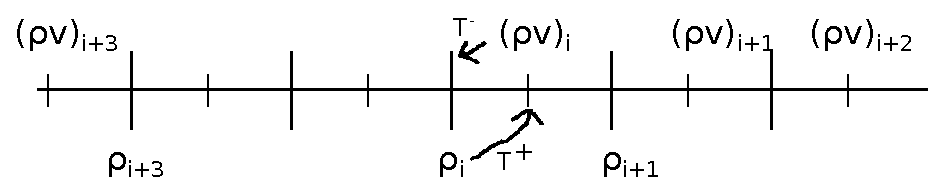
\includegraphics[width=\columnwidth]{staggered.eps}
    \caption{Staggered grid with cyclic boundary conditions}
    \label{fig:staggered}
\end{figure}

Interpolate forward half a step ($\Delta x/2$):
\begin{align}
    T^+_x(\mathbf{g}(x, y, z, \cdots)) &=  \mathbf{g}(x+1/2 \Delta x, y, z, \cdots) = \mathbf{g}_{x+1/2} \\
    &= a(\mathbf{g}_{x} + \mathbf{g}_{x+1}) + b\left( \mathbf{g}_{x-1} \mathbf{g}_{x+2} \right) + c \left( \mathbf{g}_{x-2} + \mathbf{g}_{x+3} \right) \\
    & = 
    \begin{bmatrix}
        a \quad b \quad c
    \end{bmatrix}
    \cdot
    \begin{bmatrix}
        \mathbf{g}_x + \mathbf{g}_{x+1} \\
        \mathbf{g}_{x-1} + \mathbf{g}_{x+2} \\
        \mathbf{g}_{x-2} + \mathbf{g}_{x+3}
    \end{bmatrix}
    \label{eq:interp}
\end{align}
\begin{align*}
    a &= \frac{1}{2} - b - c; \qquad b = -\frac{1}{24} - 5c; \qquad c = \frac{3}{640} 
\end{align*}

    
\end{frame}
\begin{frame}[shrink=20]

\frametitle{Solving in space}

\begin{align}
    T^+_x(\mathbf{g}(x, y, z, \cdots)) &=  \mathbf{g}_{x+1/2} = 
    \begin{bmatrix}
        a \quad b \quad c
    \end{bmatrix}
    \cdot
    \begin{bmatrix}
        \mathbf{g}_x + \mathbf{g}_{x+1} \\
        \mathbf{g}_{x-1} + \mathbf{g}_{x+2} \\
        \mathbf{g}_{x-2} + \mathbf{g}_{x+3}
    \end{bmatrix}
\end{align}
\begin{align}
    \partial^+_{,x}(\mathbf{g}(x, y, z, \cdots)) &=  \mathbf{g}_{x+1/2}' = 
    \begin{bmatrix}
        a' \quad b' \quad c'
    \end{bmatrix}
    \cdot
    \begin{bmatrix}
        \mathbf{g}_x - \mathbf{g}_{x+1} \\
        \mathbf{g}_{x-1} - \mathbf{g}_{x+2} \\
        \mathbf{g}_{x-2} - \mathbf{g}_{x+3}
    \end{bmatrix}
    \label{eq:deriv}
\end{align}

\begin{figure}[htpb]
    \centering
    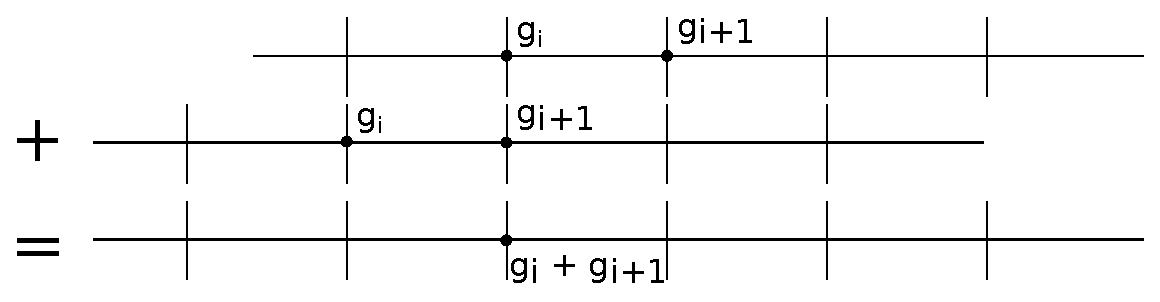
\includegraphics[width=\columnwidth]{roll.eps}
    \caption{Numpy's \texttt{ROLL(array, steps)} causing cyclic boundaries, using this to interpolate and differentiate}
    \label{fig:roll}
\end{figure}

\end{frame}

\subsection{Equations restated}
\begin{frame}
    \frametitle{Equations restated}

    Solve only for momentum $\rho v$ and density $\rho$, meaning the velocity can be found (at $\rho v$'s location):
    \begin{equation}
        v = \frac{\rho v}{T^+_z \left[ \rho \right]}
        \label{eq:vel}
    \end{equation}

    Momentum equation
    \begin{equation}
        \frac{\partial \rho v}{\partial t} = -\partial_{,z}^+ \left[ \frac{1}{\rho} \left( T^{-}_z \left( \left( \rho v \right)^2 \right) \right) \right] + \partial^+_{,z} \left[ p_{\rm gas} + Q \right] + T^+_z \left[ \rho \right] g_z
        \label{eq:staggered_momentum}
    \end{equation}

    Mass continuity equation
    \begin{equation}
        \frac{\partial \rho}{\partial t} = - \partial^-_{,z} \left[ \rho v \right]
        \label{eq:staggered_density}
    \end{equation}

\end{frame}

\section{Results}
\subsection{Stability check}
\begin{frame}
    \frametitle{Stability check}
    \href{http://77.237.250.152/wordpress/studier/stability_web.mp4}[\beamergotobutton{http://77.237.250.152/wordpress/studier/stability\_web.mp4}]

    \begin{center}
\includemedia[
width=0.8\linewidth,height=0.6\linewidth, % 16:9
activate=pageopen,
flashvars={
modestbranding=1 % no YT logo in control bar
&autohide=1 % controlbar autohide
&showinfo=0 % no title and other info before start
&rel=0          % no related videos after end
}
]{}{http://www.youtube.com/v/pQj6pArdMPc?rel=0}
    \end{center}


\end{frame}

\subsection{Stable without pressure}
\begin{frame}
    \frametitle{Stable without pressure}
    \href{http://77.237.250.152/wordpress/studier/alive.mp4}[\beamergotobutton{http://77.237.250.152/wordpress/studier/alive.mp4}]

    \begin{center}
\includemedia[
width=0.8\linewidth,height=0.6\linewidth, % 16:9
activate=pageopen,
flashvars={
modestbranding=1 % no YT logo in control bar
&autohide=1 % controlbar autohide
&showinfo=0 % no title and other info before start
&rel=0          % no related videos after end
}
]{}{http://www.youtube.com/v/z0xPSETtJpA?rel=0}
    \end{center}

\end{frame}

\subsection{Stable for small amplitudes}
\begin{frame}
    \frametitle{Stable for small amplitudes}
    \href{http://77.237.250.152/wordpress/studier/working.mp4}[\beamergotobutton{http://77.237.250.152/wordpress/studier/working.mp4}]

    \begin{center}
\includemedia[
width=0.8\linewidth,height=0.6\linewidth, % 16:9
activate=pageopen,
flashvars={
modestbranding=1 % no YT logo in control bar
&autohide=1 % controlbar autohide
&showinfo=0 % no title and other info before start
&rel=0          % no related videos after end
}
]{}{http://www.youtube.com/v/f6XDzfA12eE?rel=0}
    \end{center}


\end{frame}

\section{To do}
\subsection{To do}
\begin{frame}
    \frametitle{To do:}

    \begin{enumerate}
        \item Remember. There is no such thing as negative density
        \item Try with sine peak as initial condition for $\rho$
        \item Try to get the artificial diffusion implemented:
            \begin{equation}
                \del \cdot \mathbf{t} = \del \cdot \mathbf{Q} \stackrel{\text{\small 1D}}{=} \mu \frac{\diffd v}{dx}
                \label{eq:diffusion}
            \end{equation}
            with $\mu = \rho c_s \lambda$ and $\lambda = \nu \Delta x$.
        \item Don't forget that there's no such thing as negative density
    \end{enumerate}

\end{frame}

\subsection{Stagger code}
\begin{frame}[fragile,shrink=40]
    \frametitle{\texttt{stagger.py}}
    \lstinputlisting{../exercises2/stagger.py}
\end{frame}

\begin{frame}
    \frametitle{What happens when you have negative density}
    \href{http://77.237.250.152/wordpress/studier/blowup_web.mp4}[\beamergotobutton{http://77.237.250.152/wordpress/studier/blowup\_web.mp4}]

    \begin{center}
\includemedia[
width=0.8\linewidth,height=0.6\linewidth, % 16:9
activate=pageopen,
flashvars={
modestbranding=1 % no YT logo in control bar
&autohide=1 % controlbar autohide
&showinfo=0 % no title and other info before start
&rel=0          % no related videos after end
}
]{}{http://www.youtube.com/v/mKcvXZ2biQI?rel=0}
    \end{center}


\end{frame}

%------------------------------------------------


\end{document}
